\selectlanguage{english}
\setlength{\parindent}{0.5cm}
\section{RNN Architectures}
Even though the RNN can discover the long-term dependencies,
it could be difficult to train an effective RNN model using gradient descent
as stated by Bengio et al. (1994) \cite{bengio1994learning} and Hochreiter et al. (2001) \cite{hochreiter2001gradient}.
As a result, RNN architecture has been revised in various ways for the past decade.
A wide range of configurations is proposed such as the change 
of activation gate, the addition of bias linear equation term, etc. 
Hochreiter and Schmidhuber (1997) \cite{journals/neco/HochreiterS97} proposed a well-known architecture called
Long Short-Term Memory (LSTM).
Cho et al. (2014) \cite{cho2014learning} proposed another RNN model called Gated Recurrent Unit (GRU). 
It is proved that these models have the ability to solve the vanishing gradient problem.
Thus, various kinds of LSTM and GRU architectures were commonly used instead of default RNN.
Since LSTM has the highest numbers of parameters, 
it has more advantages than other RNN architectures because of the adjustment variation.
The LSTM and GRU architectures used in this paper are discussed in the following subsections.

\subsection{Long Short-Term Memory (LSTM)}
\begin{figure}[!h]
\centering
  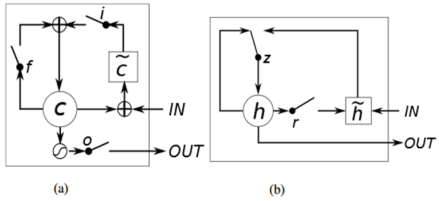
\includegraphics[scale=1]{image/lstm_struc.png}
  \caption{Illustration of LSTM (a) and GRU (b).}
  \label{fig:1}
\end{figure}
As shown in Figure~\ref{fig:1} (a), LSTM contains three gates: forget gate ($f_t$), input gate ($i_t$) 
and output gate ($o_t$). 
The $o_t$ is connected to the cell state ($C_t$) that carries out the error 
back through time. Equations~\ref{eq:1}-\ref{eq:6} show how to update a forget gate, 
an input gate, an output gate, a candidate cell state, a cell state and a hidden unit, 
respectively. 
The variables $w_{xy}$, $h$, $b$, $\bar{C_t}$ stand for weight of gates, 
hidden unit weights, bias and a candidate of a cell state respectively. 
Finally, $t$ and $\sigma$ stands for time domain and activation function.
 
\begin{equation}
f_t=\sigma(w_{xf}x_t+w_{hf}h_{t-1}+b_f)
\label{eq:1}
\end{equation}
\begin{equation}
i_t=\sigma(w_{xi}x_t+w_{hi}h_{t-1}+b_i)
\label{eq:2}
\end{equation}
\begin{equation}
o_t=\sigma(w_{xo}x_t+w_{ho}h_{t-1}+b_o)
\label{eq:3}
\end{equation}
\begin{equation}
\bar{C_t}=\sigma(w_{xc}x_t+w_{hc}h_{t-1}+b_c)
\label{eq:4}
\end{equation}
\begin{equation}
C_t=f_t \cdot C_{t-1}+i_t \cdot \bar{C_t}
\label{eq:5}
\end{equation}
\begin{equation}
h_t  = o_t\cdot \sigma(C_t)
\label{eq:6}
\end{equation}


\subsection{Long Short-Term Memory (LSTM)}
As shown in Figure~\ref{fig:1} (b), GRU contains one less gate than LSTM. 
Indeed, it has only reset and update gates.
This is almost equivalent to LSTM Coupling Input Forget Gates (LSTM-CIFG)
except that it merges cell state and hidden state into one parameter. 
Equations~\ref{eq:7}-\ref{eq:10} show how to update an update gate ($z$), 
a reset gate ($r$), a hidden gate ($h$) and a cell state ($s_t$), 
respectively. The variables $U$ and $W$ are input weight and hidden weight, 
which are the training parameters. The variable $x$ is the input while $s$ 
is the state parameter in a time domain $t$. $\sigma$ stands for activation function.
\begin{equation}
z = \sigma(x_tU^z+s_{t-1}W^z)
\label{eq:7}
\end{equation}
\begin{equation}
r = \sigma(x_tU^r+s_{t-1}W^r)
\label{eq:8}
\end{equation}
\begin{equation}
h = \sigma(x_tU^h+(s_{t-1} \cdot r)W^h)
\label{eq:9}
\end{equation}
\begin{equation}
s_t  = \sigma((1-z)\cdot h)+(s_{t-1} \cdot z)
\label{eq:10}
\end{equation}

\subsection{Variation of LSTM}
Various LSTM architectures have been introduced recently.
However, we discuss only the variations that are used in our work: 
Coupled In-put and Forget Gate (CIFG), peephole, and Full Gate Recurrence 
(FGR). The equations of the three architectures are shown below, 
which are based on Greff et al. (2015) \cite{greff2017lstm}
with slightly modification in FGR by removing peephole from the equation.
First, CIFG is the easiest to implement and is the most similar to GRU architecture.
The equation of CIFG is almost the same as default LSTM except that
we intend to use input gate and forget gate together. 
Therefore, the equation of the forget gate is changed as in Equation~\ref{eq:11}.

\begin{equation}
f_t  = \sigma(1-i_t)
\label{eq:11}
\end{equation}
Second, the LSTM peephole (Gers and Schmidhuber, 2000; Graves et al. 2009)
\cite{gers2000recurrent,graves2009novel}
improves the ability of LSTM to learn the model that requires 
precise timing and counting of the internal states.
The concept for this architecture is to enable the gate to peek
into the previous cell state. 
Therefore, another $p$ term is added into the equation of all gates as follows.
\begin{equation}
f_t=\sigma(w_{xf}x_t+w_{hf}h_{t-1}+p_fC_{t-1}+b_f)
\label{eq:12}
\end{equation}
\begin{equation}
i_t=\sigma(w_{xi}x_t+w_{hi}h_{t-1}+p_iC_{t-1}+b_i)
\label{eq:13}
\end{equation}
\begin{equation}
o_t=\sigma(w_{xo}x_t+w_{ho}h_{t-1}+p_oC_{t-1}+b_o)
\label{eq:14}
\end{equation}
Finally, FGR is the most complex architecture that allows each gate in the previous
state to interact with itself in the next state as shown in
Equation~\ref{eq:15}-\ref{eq:20}.
The variables $\bar{f_t}$, $\bar{i_t}$t, and $\bar{o_t}$t are candidate 
of the forget gate, input gate, output gate respectively
that will be summed with other product of recurrence terms.
The recurrence terms R is interaction with each gate of the previous state.
\begin{equation}
\bar{f_t}=(w_{xf}x_t+w_{hf}h_{t-1}+b_f)
\label{eq:15}
\end{equation}
\begin{equation}
\bar{i_t}=(w_{xi}x_t+w_{hi}h_{t-1}+b_i)
\label{eq:16}
\end{equation}
\begin{equation}
\bar{o_t}=(w_{xo}x_t+w_{ho}h_{t-1}+b_o)
\label{eq:17}
\end{equation}
\begin{equation}
f_t = \sigma(\bar{f_t}+R_{if}i_{t-1}+R_{ff}f_{t-1}+R_{of}o_{t-1})
\label{eq:18}
\end{equation}
\begin{equation}
i_t = \sigma(\bar{i_t}+R_{ii}i_{t-1}+R_{fi}f_{t-1}+R_{oi}o_{t-1})
\label{eq:19}
\end{equation}
\begin{equation}
o_t = \sigma(\bar{o_t}+R_{io}i_{t-1}+R_{fo}f_{t-1}+R_{oo}o_{t-1})
\label{eq:20}
\end{equation}

\subsection{Bi-directional RNN}
The direction of the dependency between the words in the text
is not only forward but also backward. 
Therefore, bi-directional model is usually applied to 
capture these forward and backward dependencies. 
Schuster and Paliwal (1997) \cite{schuster1997bidirectional} invented 
the model by connected two hidden layers of opposite directions to the same
output as shown in Figure~\ref{fig:2}. 
It was successfully applied in various NLP tasks such as character
modeling (Ling et al. 2015) \cite{ling2015finding}
and encoding of the words and sentences.
\begin{figure}[!h]
\centering
  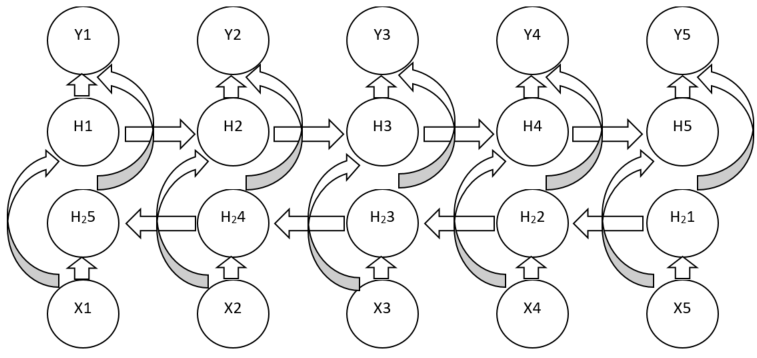
\includegraphics[scale=0.8]{image/birnn.png}
  \caption{Bi-directional RNN.}
  \label{fig:2}
\end{figure}